In diesem Kapitel wollen wir für Prozesse auf einem endlichen Wahrscheinlichkeitsraum eine Möglichkeit herleiten, die adaptierte Wasserstein-Metrik tatsächlich auszurechnen. Wir betrachten also Prozesse 
$$\mathbb{X} = \left( \Omega^\mathbb{X}, \mathcal{F}^\mathbb{X}, \mathbb{P}^\mathbb{X}, (\mathcal{F}_t^\mathbb{X})_{t=1}^N, (X_t)_{t=1}^N\right)$$
mit $|\Omega^\mathbb{X}| < \infty$. Als direkte Konsequenz sind auch die $\mathcal{F}_t^\mathbb{X}$ endlich. Wir schreiben $\mathcal{E}_t^\mathbb{X}$ für die \emph{Atome} von $\mathcal{F}_t^\mathbb{X}$, das heißt
$$\mathcal{E}_t^\mathbb{X} := \left\{A \in \mathcal{F}_t^\mathbb{X}  \vert \nexists B \in \mathcal{F}_t^\mathbb{X}: \emptyset \subsetneq B \subsetneq A \right\} \setminus \{\emptyset\}$$
Da $\mathcal{F}_t^\mathbb{X}$ stabil unter Schnitten ist, sind die Mengen in $\mathcal{E}_t^\mathbb{X}$ disjunkt. Weiterhin kann man jedes Element $A \in \mathcal{F}_t^\mathbb{X}$ schreiben als 
$$A = \bigsqcup_{B \in \mathcal{E}_t^\mathbb{X}, B \subseteq A} B$$
Das sieht man zum Beispiel durch Induktion über die Größen von Mengen in $\mathcal{F}_t^\mathbb{X}$: Mengen der Kardinalität $1$ können keine echten Teilmengen haben und sind also in $\mathcal{E}_t^\mathbb{X}$ enthalten. Wenn die Aussage nun für alle Mengen von Kardinalität $\leq n$ gilt, so gilt für eine Menge $A \in \mathcal{F}_t^\mathbb{X}$ der Kardinalität $n+1$: Entweder hat $A$ keine echten Teilmengen, also $A \in \mathcal{E}_t^\mathbb{X}$, oder $A$ hat mindestens eine solche echte Teilmenge $B \in \mathcal{F}_t^\mathbb{X}$. Dann ist $A=A\cap B \cup A \setminus B$ und beide von diesen Mengen sind nach Induktionsvoraussetzung darstellbar. Somit folgt auch die Darstellbarkeit von $A$. Wir bezeichnen diese Eigenschaft der $\sigma$-Algebren als \emph{atomar}.

Um die Implementierung der adaptierten Wasserstein-Metrik besser zu verstehen betrachten wir zunächst eine Möglichkeit zur Implementierung der klassischen Wasserstein-Metrik auf einem endlichen Wahrscheinlichkeitsraum, denn viele der Ideen sind direkt übertragbar.

\subsection{Klassische Wasserstein-Metrik}
Die Berechnung der Wasserstein-Metrik $\mathcal{W}_p$ zwischen zwei Verteilungen $\mu, \nu$ auf einem metrischen Raum $(\Omega, d)$, $\Omega=\{1,...,n\}$ lässt sich als folgendes Problem darstellen: Wir suchen eine Matrix $\pi \in \mathbb{R}_{\geq 0}^{n\times n}$ mit den Eigenschaften
\begin{itemize}
    \item $\sum_{1\leq i\leq n} \sum_{1\leq j \leq n} \pi(i,j) = 1$
    \item $\sum_{1\leq i \leq n} \pi(i,j) = \nu(j) \quad\forall 1\leq j \leq n$
    \item $\sum_{1\leq j \leq n} \pi(i,j) = \mu(i) \quad\forall 1\leq i \leq n$
\end{itemize}
die den Term
$$c(\pi) = \sum_{1\leq i,j\leq n} \pi(i,j) d^p(i,j)$$ 
minimiert. Das ist ein \emph{lineares Problem}: Wenn wir $\pi$ als Element in $\mathbb{R}_{\geq 0}^{n^2}$ auffassen, so ist $c(\pi) = \langle \pi, c \rangle$ für den Vektor $c=(d^p(i,j))_{1\leq i,j\leq n}$ und auch die Nebenbedingungen sind in dieser Weise linear in den Einträgen von $\pi$: Die erste Nebenbedingung ist zum Beispiel der Form $\langle \pi, (1)_{1\leq i,j\leq n}\rangle = 1$, und die Nebenbedingungen des zweiten Punkts sind der Form  $\langle \pi, (\delta_{j_0j})_{1\leq i,j\leq n}\rangle = \nu(j_0)$ für die verschiedenen $j_0$.

Wenn wir nun also alle Vektoren aus diesen $m:=2n+1$ Nebenbedingungen in einer Matrix $A \in \mathbb{R}^{m \times n^2}$ sammeln und die Gleichheitsvorschriften der Nebenbedingungen (also zum Beispiel die Zahl 1 für die erste Nebenbedingung oder die Zahl $\nu(1)$ für eine der zweiten Nebenbedingungen) in einem Vektor $b \in \mathbb{R}^m$ zusammenfügen, so ist das Problem eine Minimierung von $\langle \pi, c\rangle$ unter den Nebenbedingungen $\pi \geq 0$ und $A\pi = b$. Das ist genau die Formulierung eines Problems für \emph{lineare Programmierung} und kann mit bekannten Methoden gelöst werden. \footnote{In klassischen Formulierungen sind manchmal nur Nebenbedingungen der Form $Ax \leq b$ erlaubt. Das ist aber kein Problem, da $Ax=b$ genau dann gilt, wenn $Ax\leq b$ und $(-A)x \leq -b$. Wir können also auch nur durch $Ax \leq b$ Gleichheiten darstellen, indem wir die Anzahl der Nebenbedingungen verdoppeln. }%TODO: Bekannte Methoden referenzieren

Wir können aber die Anzahl der Nebenbedingungen noch reduzieren: Die drei Nebenbedingungen oben sind äquivalent zu 
\begin{itemize}
    \item $\sum_{1\leq j \leq n} \pi(i,j) \leq \mu(i) \quad \forall 1\leq i\leq n$
    \item $\sum_{1\leq i \leq n} \pi(i,j) \geq \nu(j) \quad \forall 1\leq j\leq n$
\end{itemize}
da aus diesen zwei Bedingungen bereits folgt 
$$\sum_{1\leq i\leq n} \sum_{1\leq j\leq n} \pi(i,j) \leq \sum_{1\leq i\leq n} \mu(i) = 1$$
und gleichzeitig
$$\sum_{1\leq j\leq n}\sum_{1\leq i\leq n} \pi(i,j) \geq \sum_{1\leq j\leq n}\nu(j)=1$$
weshalb an jeder Stelle Gleichheit gelten muss.

Wir konnten also das Berechnen der Wasserstein-Metrik als lineares Problem mit $2n$ Ungleichungen als Nebenbedingung formulieren. Zu beachten ist auch, dass in jeder Nebenbedingung nur das Äquivalent von einer Zeile bzw. Spalte von $\pi$ eine 1 enthält, der Rest besteht aus Nullen. Die Matrix $A$ ist also dünnbesetzt mit einem Anteil von $\frac{1}{n}$ an Nicht-Null-Einträgen.

\subsection{Adaptierte Wasserstein-Metrik}
Wir wollen nun Überlegungen zur Berechnung der adaptierten Wasserstein-Metrik anstellen. Von der Methodik her verläuft das sehr ähnlich wie für die klassische Wasserstein-Metrik: Zusätzlich zu den Nebenbedingungen aus dem letzten Abschnitt wollen wir nun auch die Eigenschaft von \emph{Bikausalität} einer Kopplung durch möglichst wenig lineare Nebenbedingungen ausdrücken. 

Wir betrachten zunächst die Anforderung an Kausalität für eine Kopplung $\pi \in \cpl(\mathbb{X}, \mathbb{Y})$ zweier filtrierter Prozesse auf endlichen Räumen $\Omega^\mathbb{X}$ und $\Omega^\mathbb{Y}$. 

\begin{lemma}\label{thm:causality_finite_case}
    $\pi$ ist kausal genau dann, wenn für alle $1\leq t < N$, $B \in \mathcal{E}_t^\mathbb{Y}, C \in \mathcal{E}_t^\mathbb{X}$ und $A \in \mathcal{E}_{t+1}^\mathbb{X}$ mit $A \subseteq C$ gilt
    $$\sum_{(x,y) \in A\times B} \pi(x,y)\mathbb{P}^\mathbb{X}(C) = \sum_{(x,y) \in C\times B} \pi(x,y) \mathbb{P}^\mathbb{X}(A)$$
\end{lemma}
\begin{proof}
Zur Vereinfachung der Notation schreiben wir an vielen Stellen in diesem Beweis etwa nur $B$ statt $\Omega^\mathbb{X} \times B$, wenn aus dem Kontext klar ist, welche Koordinate gemeint ist. Nach Lemma \ref{thm:causality_characterization} ist $\pi$ kausal genau dann, wenn für alle $1\leq t < N$ und $B \in \mathcal{F}_t^\mathbb{Y}$ gilt 
\begin{equation}\label{eq:71_00}
    \mathbb{E}_\pi(\mathds{1}_B \vert \mathcal{F}_{N,0}^{\mathbb{X,Y}}) = \mathbb{E}_\pi(\mathds{1}_B \vert \mathcal{F}_{t,0}^{\mathbb{X,Y}})
\end{equation}
Die $\sigma$-Algebren $\mathcal{F}_{t,0}^{\mathbb{X,Y}}$ werden erzeugt von den disjunkten Mengen $\{A\times \Omega^\mathbb{Y} \vert A \in \mathcal{E}_t^\mathbb{X}\}$. Für diesen Fall einer atomaren $\sigma$-Algebra können wir die bedingte Erwartung konkret angeben als
\begin{equation}\label{eq:71_01}
    \mathbb{E}_\pi(\mathds{1}_B \vert \mathcal{F}_{t,0}^{\mathbb{X,Y}}) = \sum_{A \in \mathcal{E}_t^\mathbb{X}, \mathbb{P}^\mathbb{X}(A)>0} \pi(B \vert A) \mathds{1}_{A}
\end{equation}
Dass der rechte Term messbar bezüglich $\mathcal{F}_{t,0}^{\mathbb{X,Y}}$ ist, ist evident, und für Mengen $D \in \mathcal{F}_t^\mathbb{X}$ ist 
\begin{align*}
    \mathbb{E}\left( \mathds{1}_D\left( \sum_{A \in \mathcal{E}_t^\mathbb{X}, \mathbb{P}^\mathbb{X}(A)>0} \pi(B \vert A) \mathds{1}_{A}\right)\right) &= \mathbb{E}\left( \sum_{A \in \mathcal{E}_t^\mathbb{X}, \mathbb{P}^\mathbb{X}(A)>0, A\subseteq D} \pi(B \vert A) \mathds{1}_{A}\right) \\
    &= \sum_{A \in \mathcal{E}_t^\mathbb{X}, \mathbb{P}^\mathbb{X}(A)>0, A\subseteq D} \pi(B\cap A) \\
    &= \pi\left( B\cap \bigsqcup_{A \in \mathcal{E}_t^\mathbb{X}, A\subseteq D}A\right) \\
    &= \pi(D \cap B)
\end{align*}
Somit gilt Gleichung \ref{eq:71_01} also tatsächlich. Damit nun Gleichung \ref{eq:71_00} erfüllt wird, muss genau gelten
$$\sum_{C \in \mathcal{E}_t^\mathbb{X}, \mathbb{P}^\mathbb{X}(C)>0} \pi(B \vert C) \mathds{1}_C = \sum_{A \in \mathcal{E}_N^\mathbb{X}, \mathbb{P}^\mathbb{X}(A)>0} \pi(B \vert A) \mathds{1}_A \quad \text{ fast sicher }$$
Diese Gleichheit gilt genau dann, wenn für alle $B \in \mathcal{F}_t^\mathbb{Y}$, alle $A \in \mathcal{E}_N^\mathbb{X}$ mit $\mathbb{P}^\mathbb{X}(A)>0$ und für die eindeutige Obermenge $C \in \mathcal{E}_t^\mathbb{X}$ mit $A\subseteq C$ gilt $\pi(B\vert A) = \pi(B \vert C)$ oder äquivalent
\begin{equation}\label{eq:71_02}
    \pi(B\cap A) \mathbb{P}^\mathbb{X}(C) = \pi(B\cap C) \mathbb{P}^{\mathbb{X}}(A)
\end{equation}
Jede Menge $B \in \mathcal{F}_t^\mathbb{Y}$ ist der Form
$$B = \bigsqcup_{i=1}^{n}B_i, B_1,...,B_n \in \mathcal{E}_t^\mathbb{Y}, n \in \mathbb{N}$$
Gleichung \ref{eq:71_02} ist dann 
$$\sum_{1\leq i\leq n} \pi(B_i \cap A) \mathbb{P}^\mathbb{X}(C) = \sum_{1\leq i\leq n}\pi(B_i \cap C) \mathbb{P}^\mathbb{X}(A)$$
Damit ist es hinreichend (und notwendig), die Bedingung für $B \in \mathcal{E}_t^\mathbb{Y}$ zu prüfen. 

Es ist also $\pi \in \cplc(\mathbb{X}, \mathbb{Y})$ genau dann, wenn für alle $1\leq t<N$, $B \in \mathcal{E}_t^\mathbb{Y}, C \in \mathcal{E}_t^\mathbb{X}, A \in \mathcal{E}_N^\mathbb{X}$ mit $A \subseteq C$ gilt
\begin{equation}\label{eq:71_03}
    \pi(B \cap A) \mathbb{P}^\mathbb{X}(C) = \pi(B\cap C) \mathbb{P}^\mathbb{X}(A)
\end{equation}
Wir zeigen, dass Gleichung \ref{eq:71_03} genau dann gilt, wenn sie für $A \in \mathcal{E}_{t+1}^\mathbb{X}, A \subseteq C$ gilt. 

Für die Hinrichtung sei $A \in \mathcal{E}_{t+1}^\mathbb{X}$ mit $A \subseteq C$. Dann ist $A$ der Form $A = \sqcup_{i=1}^{n} A_i$ für $A_i \in \mathcal{E}_N^\mathbb{X}$ mit $A_i \subseteq A \subseteq C$. 
Somit folgt
$$\pi(B\cap A)\mathbb{P}^\mathbb{X}(C) = \sum_{i=1}^n\pi(B\cap A_i) \mathbb{P}^\mathbb{X}(C) = \sum_{i=1}^n\pi(B\cap C) \mathbb{P}^{\mathbb{X}}(A_i) = \pi(B \cap C) \mathbb{P}^\mathbb{X}(A)$$

Für die Rückrichtung zeigen wir induktiv für $1 \leq s\leq N-t$, dass Gleichung \ref{eq:71_03} für $A \in \mathcal{E}_{t+s}^\mathbb{X}, A\subseteq C$ gilt. Der Induktionsanfang $s=1$ ist genau die Voraussetzung. Gelte nun die Behauptung für ein festes $s$ und sei $A \in \mathcal{E}_{t+s+1}^\mathbb{X}$ mit $A \subseteq C$. Falls $\mathbb{P}^\mathbb{X}(A)=0$ gilt Gleichung \ref{eq:71_03} für $A$. Andernfalls ist die Gleichung äquivalent zu 
$$\pi(B \vert C) = \pi(B \vert A)$$
Bezeichne mit $A' \subseteq C$ die Obermenge von $A$ in $\mathcal{E}_{t+s}^\mathbb{X}$. Nach Induktionsvoraussetzung gilt (da $\mathbb{P}^\mathbb{X}(A') \geq \mathbb{P}^\mathbb{X}(A)> 0$)
\begin{equation}\label{eq:71_last}
    \pi(B \vert C) = \pi(B \vert A')
\end{equation}
Weiterhin ist $B = \bigsqcup_{i=1}^n B_i$ für $B_i \in \mathcal{E}_{t+s}^\mathbb{Y}$ und aus dem Fall $s=1$ (und $t \rightarrow t+s$) folgt
$$\pi(B \vert A') = \sum_{i=1}^n \pi(B_i \vert A') = \sum_{i=1}^n \pi(B_i \vert A) = \pi(B \vert A)$$
Zusammen mit Gleichung \ref{eq:71_last} gilt
$$\pi(B \vert C) = \pi(B \vert A)$$
Hieraus folgt die Induktionsbehauptung und damit auch schon die gesamte Behauptung.
\end{proof}
\begin{remark}
    Im letzten Beweis hätten wir auch bei der Bedingung mit $A \in \mathcal{E}_N^\mathbb{X}$ bleiben können. Wenn wir zum Beispiel Münzwürfe mit natürlicher Filtration betrachten, dann hat $\mathcal{E}_t^\mathbb{X}$ $2^t$ Elemente mit jeweils $2$ direkten Kindern und $2^{N-t}$ Blättern. Wir hätten also bei der Variante mit $\mathcal{E}_N^\mathbb{X}$ 
    $$\sum_{k=0}^{N-1} 2^k2^{N-k}2^k=2^N(2^N-1) \approx 4^N$$
    Gleichungen und mit der zweiten Variante
    $$\sum_{k=0}^{N-1} 2^k22^k = 2\frac{4^N-1}{3} \approx \frac{2}{3}4^N$$
    Gleichungen. Wir haben also nur eine Einsparung in linearer Größenordnung. Die weitere Umformung zu einer Bedingung an $\mathcal{E}_{t+1}^\mathbb{X}$ ist aber auch in der Hinsicht schön, dass sie Kausalität als eine lokale Eigenschaft ausdrückt.
\end{remark}
\begin{corollary}
Seien $\mathbb{X,Y} \in \mathcal{FP}_p$ Prozesse auf endlichen Wahrscheinlichkeitsräumen und sei $\pi \in \cpl(\mathbb{X,Y})$. Dann ist $\pi$ bikausal genau dann, wenn
$$\sum_{(x,y) \in A \times B} \pi(x,y) \mathbb{P}^\mathbb{X}(C) - \sum_{(x,y) \in C \times B} \pi(x,y) \mathbb{P}^\mathbb{X}(A)\leq 0$$
für $1\leq t < N$, $B \in \mathcal{E}_t^\mathbb{Y}$, $C \in \mathcal{E}_t^\mathbb{X}$ und $A \in \mathcal{E}_{t+1}^\mathbb{X}$ mit $A\subseteq C$ gilt, sowie
$$\sum_{(x,y) \in B' \times A'} \pi(x,y) \mathbb{P}^\mathbb{Y}(C') - \sum_{(x,y) \in B' \times C'} \pi(x,y) \mathbb{P}^\mathbb{Y}(A') \leq 0$$
für $1\leq t<N$, $B' \in \mathcal{E}_t^\mathbb{X}$, $C' \in \mathcal{E}_t^\mathbb{Y}$ und $A' \in \mathcal{E}_{t+1}^\mathbb{Y}$ mit $A'\subseteq C'$ gilt.
\end{corollary}\label{thm:bicausality_finite_case}
\begin{proof}
    Bis auf den Übergang von einer Gleichung zu einer Ungleichung haben wir zu der Aussage aus Lemma \ref{thm:causality_finite_case} bloß die symmetrische Betrachtung von Antikausalität hinzugenommen. Wir müssen somit lediglich aus der Ungleichung die Gleichung ableiten. Seien dazu $B \in \mathcal{E}_t^\mathbb{Y}$, $C \in \mathcal{E}_t^\mathbb{X}$ und $A_1\in \mathcal{E}_{t+1}^\mathbb{X}$ mit $A_1 \subseteq C$. Wähle $A_2,...,A_n \in \mathcal{E}_{t+1}^\mathbb{X}$ mit $C = \sqcup_{i=1}^n A_i$. Wir haben nun für alle $1\leq i\leq n$
    $$\pi(A_i \times B) \mathbb{P}^\mathbb{X}(C) \leq \pi(C \times B) \mathbb{P}^\mathbb{X}(A_i)$$
    Somit ist auch 
    $$\pi(C\times B) \mathbb{P}^\mathbb{X}(C) = \sum_{i=1}^n \pi(A_i\times B) \mathbb{P}^\mathbb{X}(C) \leq \sum_{i=1}^n\pi(C\times B)\mathbb{P}^\mathbb{X}(A_i) = \pi(C\times B) \mathbb{P}^\mathbb{X}(C)$$
    Die äußeren Terme stimmen aber schon überein, somit muss in jedem Summanden Gleichheit gelten. Insbesondere ist 
    $$\pi(A_1 \times B) \mathbb{P}^\mathbb{X}(C) = \pi(C\times B) \mathbb{P}^\mathbb{X}(A_1)$$
    Analog folgt auch aus der Ungleichung für Antikausalität schon die entsprechende Gleichung.
\end{proof}

Die Bedingungen aus Korollar \ref{thm:bicausality_finite_case} sind linear in $\pi$. Zusammen mit den Bedingungen aus der klassischen Wasserdistanz können wir nun also die adaptierte Wasserstein-Metrik als ein lineares Problem formulieren: 

Wir suchen $\pi \in \mathbb{R}^{N^\mathbb{X}\times N^\mathbb{Y}} \geq 0$ ($N^\mathbb{X} := |\Omega^\mathbb{X}|, N^\mathbb{Y}:=|\Omega^\mathbb{Y}|$) mit 
\begin{itemize}
    \item $\sum_{y \in \Omega^\mathbb{Y}} \pi(x,y) \leq \mathbb{P}^\mathbb{X}(x)$ für alle $x \in \Omega^\mathbb{X}$.
    \item $\sum_{x \in \Omega^\mathbb{X}} \pi(x,y) \geq \mathbb{P}^\mathbb{Y}(y)$ für alle $y \in \Omega^\mathbb{Y}$.
    \item $\sum_{(x,y) \in A\times B} \pi(x,y) \mathbb{P}^\mathbb{X}(C) \leq \sum_{(x,y) \in C \times B} \pi(x,y) \mathbb{P}^\mathbb{X}(A)$ für alle $1 \leq t < N$, $B \in \mathcal{E}_t^\mathbb{Y}$, $C \in \mathcal{E}_t^\mathbb{X}$ und $A \in \mathcal{E}_{t+1}^\mathbb{X}$ mit $A \subset C$.
    \item $\sum_{(x,y) \in B' \times A'} \pi(x,y) \mathbb{P}^\mathbb{Y}(C') = \sum_{B' \times C'} \pi(x,y) \mathbb{P}^\mathbb{Y}(A')$ für alle $1 \leq t < N$, $B' \in \mathcal{E}_t^\mathbb{X}$, $C' \in \mathcal{E}_t^\mathbb{Y}$ und $A' \in \mathcal{E}_{t+1}^\mathbb{Y}$ mit $A' \subset C'$.
    \item $\pi$ minimiert 
    $$\sum_{x\in\Omega^\mathbb{X}, y\in \Omega^\mathbb{Y}} d^p(X(x), Y(y)) \pi(x,y)$$
\end{itemize}

Wir wollen diesen Abschnitt und die ganze Arbeit mit einem Beispiel abschließen: Für $s>0$ betrachten wir einen Zweischrittprozess. Im ersten Schritt starten wir zu 50\% in $s$ und zu 50\% in $-s$. Falls wir in $s$ gestartet sind, gehen wir im nächsten Schritt zu $1$ weiter, ansonsten zu $-1$. Modellieren können wir dies durch $\Omega = \{-1, 1\}$ mit Gleichverteilung und $X^s(\omega) = (s\cdot\omega, \omega)$. Die Prozesse werden in Abbildung \ref{fig:1} visualisiert. Wir wollen den Grenzwert dieser Prozesse für $s \rightarrow 0$ untersuchen. Ein möglicher Kandidat wäre der Prozess $Y(\omega) = (0, \omega)$ auf dem gleichen Wahrscheinlichkeitsraum. Tatsächlich ist das der Grenzwert bezüglich der Wasserstein-Metrik: Wir können $\pi := (\id, \id)_*\mathbb{P}$ als Kopplung wählen und erhalten 
$$\int d^p(X^s(\omega), Y(\omega)) \mathbb{P}(d\omega) = s^p$$
und somit $\mathcal{W}_p(X^s, Y) \leq s$.
\begin{figure}[h]
    \caption{Von links nach rechts: Visualisierungen von $X^s$ für $s=\frac{1}{2}$, $s=\frac{1}{10}$ und des möglichen Grenzwerts $Y$.}
    \centering
    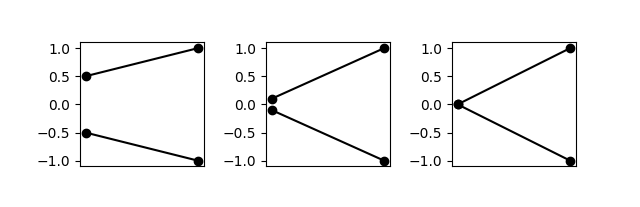
\includegraphics[width=0.8\textwidth]{process_visualization_cropped.png}
    \label{fig:1}
\end{figure}
Tatsächlich hat der Prozess $Y$ (zumindest mit natürlicher Filtration) aber ein vollkommen anderes Verhalten als $X^s$: Bei den Prozessen $X^s$ wird immer schon im ersten Schritt entschieden, zu welchem Pfad sich der Prozess entwickeln wird, wohingegen $Y$ die Entscheidung erst im zweiten Schritt trifft. Während die Wasserstein-Metrik diese Diskrepanz nicht aufzeigen konnte, ist die adaptierte Wasserstein-Metrik dazu in der Lage. Wir können die Methodik aus dem letzten Abschnitt auf die Prozesse $X^s$ und $Y$ mit natürlicher Filtration anwenden und damit die Konvergenz bezüglich $\mathcal{AW}_p$ zu untersuchen. Das Ergebnis ist in Abbildung \ref{fig:0} zu sehen. Es zeichnet sich klar ab, dass $X_s$ nicht gegen $Y$ konvergiert.
\begin{figure}[h]
    \caption{Die adaptierte Wasserstein-Distanz der Prozesse bezüglich natürlicher Filtration. Die Prozesse werden für die Folge $s_n = 2^{-n}$ aufgezeichnet.}
    \centering
    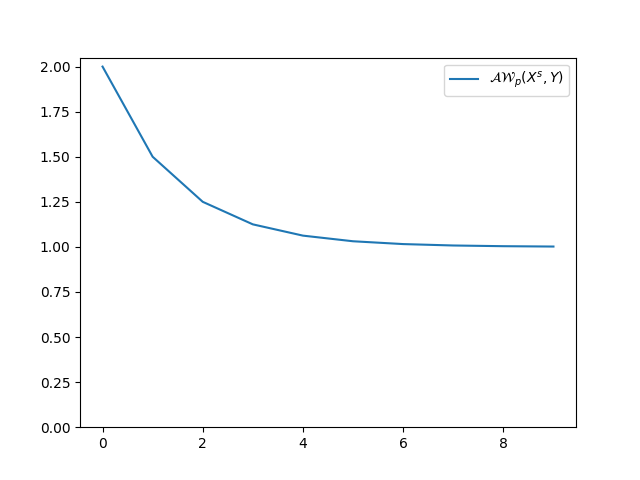
\includegraphics[width=0.7\textwidth]{aw_no_convergence.png}
    \label{fig:0}
\end{figure}

Wie wir besprochen haben ist der Hauptunterschied zwischen den Prozessen der Zeitpunkt der Entscheidung. Diese können wir aber über die Filtration darstellen: Wenn wir beim Prozess $\mathbb{Y}$ auch schon im ersten Schritt die Filtration $\mathcal{F}_1^\mathbb{Y} = \sigma(\{-1\}, \{1\})$ wählen, so sind die Filtrationen der Prozesse identisch. Damit ist die Kopplung $(\id, \id)_* \mathbb{P}$ wieder bikausal und wie bei der Wassersteindistanz konvergiert $\mathbb{X}^s \rightarrow \mathbb{Y}$ für $s \rightarrow 0$. An diesem Beispiel kann man erkennen, wie die adaptierte Wasserstein-Metrik nicht nur Nähe der Verteilungen, sondern auch Nähe des stochastischen Charakters ausdrücken kann.
